\chapter{Dynamic Programming}

\section{Longest Increasing Subsequence}

    If needed, the algorithm for LIS can be easily modified for 
    the similar task of \textbf{Longest Non-Decreasing Subsequence}.

    \kactlimport{lis.cpp}

\section{Divide-Conquer Optimization}

    Some dynamic programming problems have a recurrence of this form:

        $$ dp(i, j) = \min_{1 \leq k \leq j} dp(i - 1, k - 1) + C(k, j) $$

        where $C(k, j)$ is a cost function and $dp(i, j) = 0$ when $j \leq 0$ (using 1-idx).

        Say $ 0 \leq i < m $ and $1 \leq j \leq n$, and evaluating $C$ takes $O(1)$ time. 
        Then the straightforward evaluation of the above recurrence is $O(m n^2)$. There are
        $m \times n$ states, and $n$ transitions for each state.

        Let $opt(i, j)$ be the value of $k$ that minimizes the above expression. 
        Assuming that the cost function satisfies the quadrangle inequality, we can show that
        $opt(i, j-1) \leq opt(i, j)$ for all $i, j$. This is known as the monotonicity condition. 
        Then, we can apply divide and conquer DP. The optimal "splitting point" for a fixed 
        $i$ increases as $j$ increases.

        This lets us solve for all states more efficiently. Say we compute 
        $opt(i, j)$ for some fixed $i$ and $j$. 
        Then for any $j' < j$ we know that $opt(i, j') \leq opt(i, j)$. 
        This means when computing $opt(i, j')$, we don't have to consider as many splitting points!

        To minimize the runtime, we apply the idea behind divide and conquer. First, compute
        $opt(i, n / 2)$. Then, compute 
        $opt(i, n / 4)$, knowing that it is less than or equal to $opt(i, n / 2)$; 
        and $opt(i, 3 n / 4)$ knowing that it is greater than or equal to $opt(i, n / 2)$. 
        
        By recursively keeping track of the lower and upper bounds on 
        $opt$, we reach a $O(n \log n)$ runtime per $i$. Each possible value of $opt(i, j)$ only appears in $\log n$ different nodes.

        \kactlimport{divide-conquer-dp.cpp}

\section{Knuth Optimization}

    Knuth's optimization, also known as the Knuth-Yao Speedup, is a special case of dynamic programming on ranges, 
    that can optimize the time complexity of solutions by a linear factor, from $O(n^3)$ for standard range DP to $O(n^2)$.

    \subsection{Conditions}

        The Speedup is applied for transitions of the form:

        $$dp(i, j) = \min_{i \leq k < j} [ dp(i, k) + dp(k+1, j) + C(i, j) ].$$

        Similar to divide and conquer DP, let $opt(i, j)$ be the value of $k$ that minimizes the expression in the transition 
        ($opt$ is referred to as the "optimal splitting point" further in this article). The optimization requires that the following holds:

        $$opt(i, j-1) \leq opt(i, j) \leq opt(i+1, j).$$

        We can show that it is true when the cost function 
        $C$ satisfies the following conditions for $a \leq b \leq c \leq d$:

        $C(b, c) \leq C(a, d)$;

        $C(a, c) + C(b, d) \leq C(a, d) + C(b, c)$ (the quadrangle inequality [QI]).

        A common cost function that satisfies the above condition is the \textbf{sum of the values in a subaray}.

        \kactlimport{knuth.cpp}

\section{Slope Optimizations}

    \subsection{Convex Hull Trick}

        If multiple transitions of the DP can be seen as 
        first degree polynomials (lines). CHT can be used to optimized it

        Some valid functions:

        $ax + b$
        
        $cx^2 + ax + b$ 
        (ignore $cx^2$ if c is independent)

        \kactlimport{cht-dynamic.cpp}

    \subsection{Li-chao Tree}

        Works for any type of function that has the \textbf{transcending property}:

        Given two functions f(x),g(x) of that type, 
        if f(t) is greater than/smaller than g(t) for some x=t,
        then f(x) will be greater than/smaller than g(x) for x>t.
        In other words, once f(x) “win/lose” g(x), f(x) will continue to “win/lose” g(x).

        The most common one is the line function: $ ax + b $

    \subsection{Slope Trick}
    
    You are given an array of n integers. You want to modify the array so that it is non-decreasing, i.e., every element is at least as large as the previous element.
    On each move, you can increase or decrease the value of any element by one. What is the minimum number of moves required?
    
    \textbf{Observation: } It is also possible to solve the problem of modifying the array to stricly increasing.

    \kactlimport{slope-trick.cpp}

\section{SOS DP}

    \textbf{Sum over Subsets DP (SOS DP)} computes how many elements there are for each mask
    which are a subset of this mask.

    This can be modified for other operations in which the subset contributes for the mask
    .
    \textit{Example:}

    \textbf{10}0\textbf{1} if a subset of \textbf{11}0\textbf{1};

    \textbf{00}0\textbf{1} if a subset of \textbf{11}0\textbf{1};
    
    \textbf{11}0\textbf{0} if a subset of \textbf{11}0\textbf{1};
    
    \textbf{11}0\textbf{1} if a subset of \textbf{11}0\textbf{1};

    \begin{center}
        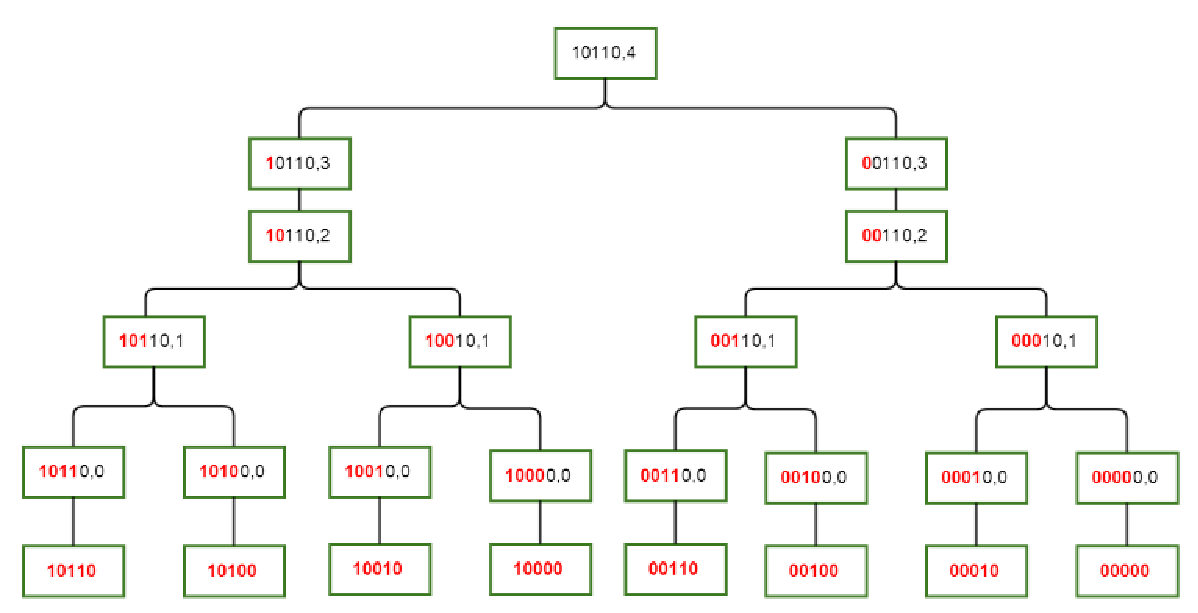
\includegraphics[width=9cm]{content/dynamic-programming/sos-example.pdf}
    \end{center}

    \kactlimport{sos-dp.cpp}